
\section{Results}\label{sec:results}
    This lab exercise was divided into four parts, each exploring the concepts described in the~\nameref{sec:theory} section.


%%%%%%%%%%%%%%%%%%%%%%%%%%%%%%%%%%%%%%%%%%%%%%%%%%%%%%%%%%%%%%%%%%%%%%%%
%%
%% Part 1
%%
%%%%%%%%%%%%%%%%%%%%%%%%%%%%%%%%%%%%%%%%%%%%%%%%%%%%%%%%%%%%%%%%%%%%%%%%

    \subsection{Part 1}\label{subsec:part1}
        This portion of the lab instructed us to create a program that conducts the following procedure in order:

        \begin{enumerate}
            \itemsep0em
            \item Declare and initialize a variable, name: "val", initial value: "0"
            \item Call \texttt{fork()}
            \item In the created child process
            \begin{enumerate}
                \itemsep0em
                \item Add "2" to the value of "val"
                \item Print "val" to console, along with the pid of the child process
            \end{enumerate}
            \item In the parent process
            \begin{enumerate}
                \itemsep0em
                \item Add "5" to the value of "val"
                \item Print "val" to console, along with the pid of the parent process
            \end{enumerate}
        \end{enumerate}
        Through this procedure we were to observe the values of the variable "val" and draw a conclusion.
        This question and its answer are provided in the~\nameref{sec:qa} section.

        \medskip
        \noindent The source code for this portion of the lab was written and compiled partially on a lab workstation and partially on a personally owned Mac.
        The code itself is included at the end of this report in Appendix~\ref{sec:part1_source}.
        Upon implementing Part 1, compiling, and running the output to console was screenshot and is as shown on the following page in Figure \ref{fig:part1_output}.

        \begin{figure}[H]
            \centering
            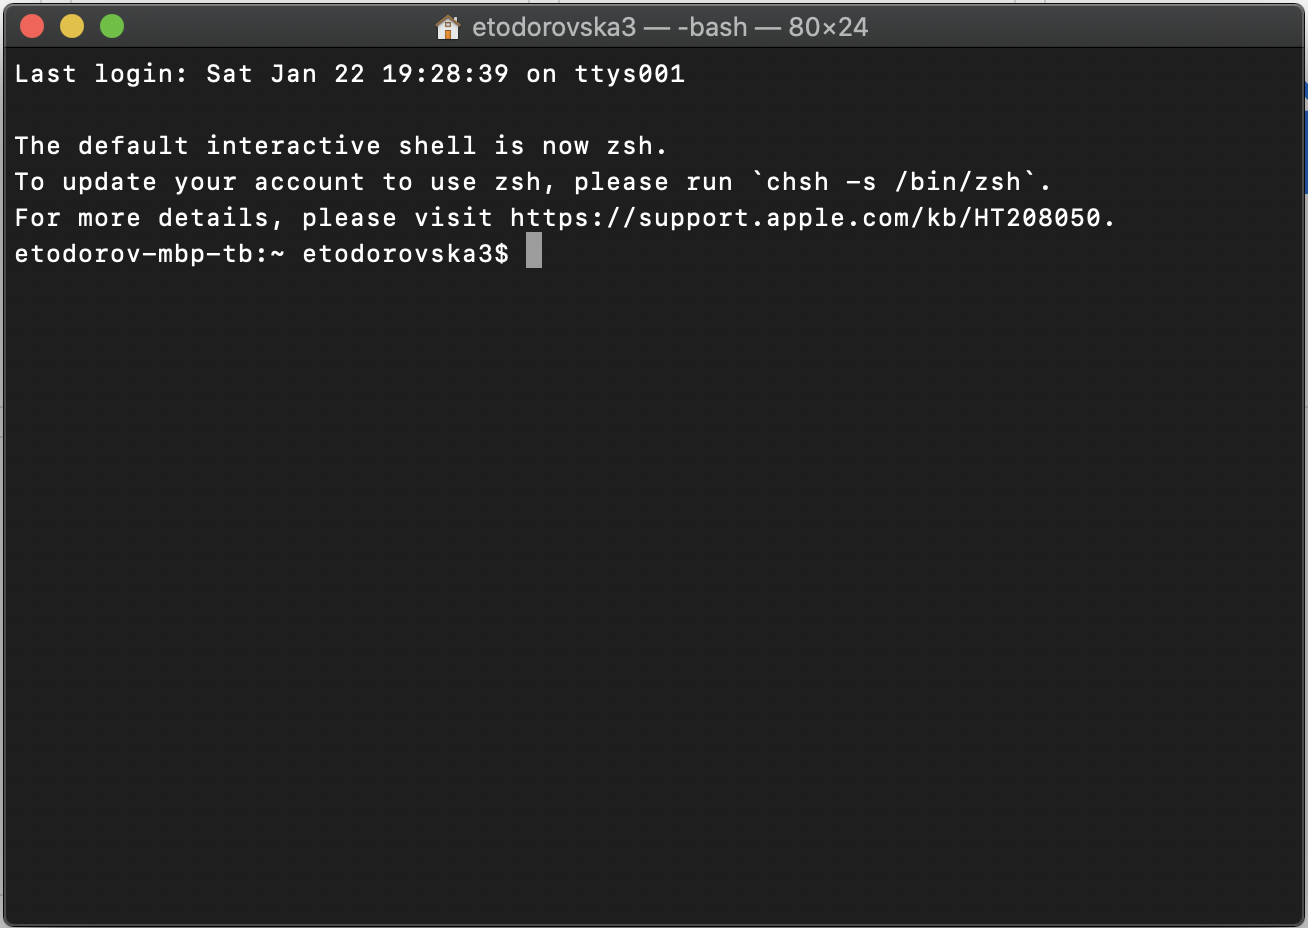
\includegraphics[width=\linewidth]{figures/placeholder.png}
            \caption{Part 1, Console Output}
            \label{fig:part1_output}
        \end{figure}
